\section{Interface 2}

\begin{figure}[!h]
    \centering{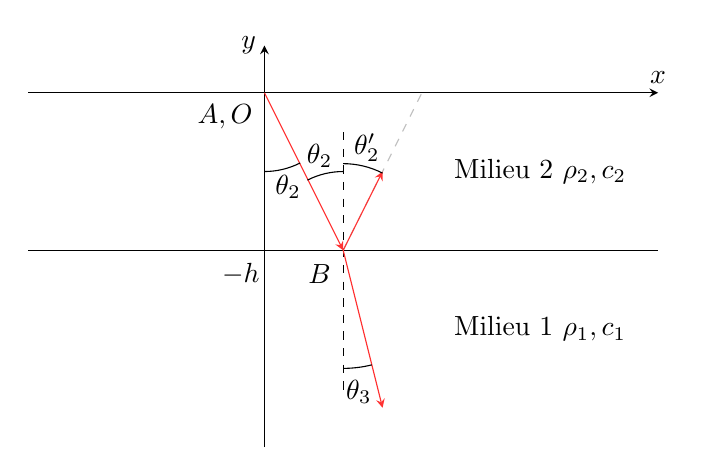
\begin{tikzpicture}

    % ifaces
    \draw [>=stealth, ->] (-3,0) -- (5,0);
    \draw (-3,-2) -- (5,-2);

    % Labels
    \draw (3.5,-1) node {Milieu 2 $\rho_2,c_2$};
    \draw (3.5,-3) node {Milieu 1 $\rho_1,c_1$};

    % verticals
    \draw [dashed] (0,.5) -- (0,-1.5);
    \draw [dashed] (1,-0.5) -- (1,-3.8);

    % axis
    %% y
    \draw [>=stealth, ->] (0,-4.5) -- (0,.6);
    \draw (-.2,.6) node {$y$};
    %% x (already drawn)
    \draw (5,.2) node {$x$};
    %% ordonnée h
    \draw (-.3,-2.3) node {$-h$};


    % points A & B
    \draw (-.5, -.3) node {$A,O$};
    \draw (.7, -2.3) node {$B$};

    % rays
    \draw [red!80, >=stealth, ->] (0,0) -- (1, -2);
    \draw [gray!50, dashed] (1,-2) -- (2,0);
    \draw [red!80, >=stealth, ->] (1,-2) -- (1.5, -1);
    \draw [red!80, >=stealth, ->] (1,-2) -- (1.5, -4);

    % angles
    \draw (0,-1) arc (-90:-63:1) node at (0.3,-1.2) {$\theta_2$};
    \draw (1,-1) arc (90:117:1) node at (.7,-.8) {$\theta_2$};
    \draw (1,-0.9) arc (90:63:1.1) node at (1.3,-.7) {$\theta_2'$};
    \draw (1,-3.5) arc (-90:-76:1.5) node at (1.2,-3.8) {$\theta_3$};


\end{tikzpicture}
}
    \caption{\label{iface2} Considération des effets à l'interface 2}
\end{figure}

Au niveau de l'interface 2 (figure~\ref{iface2}), on a exactement le même problème qu'à l'interface 1
(figure~\ref{iface1}). En fait, la distance $h$ séparant les deux interfaces a une influence uniquement dans le décalage
en $x$ du point de frappe du rayon. On exprime ce décalage $\Delta x$ ainsi :

\[
\Delta x = h\tan\theta_2
\]

De plus, d'après l'équation~\eqref{i1_snellrel}, on peut écrire :

\[
\theta_2 = \arcsin\left(\frac{k_1}{k_2}\sin\theta_1\right) \Rightarrow \Delta x = h\tan\left[\arcsin\left(\frac{k_1}{k_2}\sin\theta_1\right)\right]
\]

Ainsi, on peut utiliser un raisonnement exactement analogue à celui utilisé à l'interface 1. Pour cela considérons que
l'axe $y$ voit son origine déplacée en $B$ et re-posons notre calcul.


\subsection{Position du problème}

\paragraph{Pressions totales} Dans le milieu 2, la pression totale vérifie :

\begin{equation}
    \left(\Delta - \frac{1}{c_2^2}\frac{\partial^2}{\partial t^2}\right)\pTOT_2(x,y,t) = 0 \;;\; \forall x,t \,\mathrm{et}\, \forall y \geq 0 \label{i2_prop2}
\end{equation}


Dans le milieu 1, la pression totale vérifie :

\begin{equation}
    \left(\Delta - \frac{1}{c_1^2}\frac{\partial^2}{\partial t^2}\right)\pTOT_1(x,y,t) = 0 \;;\; \forall x,t\,\mathrm{et}\,\forall y \leq 0 \label{i2_prop2}
\end{equation}


\paragraph{Champ monochromatique} Les ondes sont considérées monochromatiques, l'équation d'Helmholtz est donc vérifiée
dans chacun des milieux :

\begin{eqnarray}
    (\Delta + k_2^2)p_2(x,y) & = & 0 \;;\; \forall x,t \label{i2_helm1}\\
    (\Delta + k_1^2)p_1(x,y) & = & 0 \;;\; \forall x,t \label{i2_helm2}
\end{eqnarray}

\paragraph{Condition de Sommerfeld}

\paragraph{Conditions à l'interface}

A l'interface, il y a continuité des pressions et des vitesses normales. Ainsi :

\begin{eqnarray}
    \pTOT_2(x, y=0, t) &=& \pTOT_1(x,y=0,t) \;;\;\forall x,t \label{i2_cl1}\\
    \vTOT_2(x, y=0, t) &=& \vTOT_1(x,y=0,t) \;;\;\forall x,t \label{i2_cl2}
\end{eqnarray}

Dans le milieu 1, on ne considérera que l'onde transmise, ainsi pour les equations~\eqref{i2_prop2},~\eqref{i2_cl1}
et~\eqref{i2_cl2}, on aura :

\begin{eqnarray*}
    \pTOT_1 = \pT_2\\
    \vTOT_1 = \vT_2
\end{eqnarray*}

On définit alors :

$$\pTOT_2 = \pI_2 + \pR_2$$

\subsection{Forme générale des pressions}

Les ondes sont considérés monochromatiques :

\begin{eqnarray}
    \pI_2(x,y,t) & = & A_2e^{j(\omega t-k_2\sin\theta_2x+k_2\cos\theta_2y)} \label{i2_pgeni}\\
    \pR_2(x,y,t) & = & B_2e^{j(\omega t-k_2\sin\theta_2'x+k_2\cos\theta_2'y)} \label{i2_pgenr}\\
    \pT_2(x,y,t) & = & A_3e^{j(\omega_3t-k_1\sin\theta_3x+k_1\cos\theta_3y)} \label{i2_pgent}
\end{eqnarray}

On remarque que $\pI_2 = \pT_1$ (voir équation~\eqref{i1_pgent}).

\subsection{Forme générales des vitesses normales}

On sait que les vitesses normales ont une expression de la forme : $v_i(x,y,t) = v_i(x,y)e^{j\omega_it}$, d'après
l'équation d'Euler, on peut écrire les équations~\eqref{i2_euler1} et \eqref{i2_euler2}.

\begin{eqnarray}
    \rho_2\frac{\partial\vTOT_2}{\partial t} = -\frac{\partial\pTOT_2}{\partial y}
        & \Leftrightarrow & \vTOT_2 = -\frac{1}{j\omega\rho_2}\frac{\partial\pTOT_2}{\partial y}\label{i2_euler1} \\
    \rho_1\frac{\partial\vT_2}{\partial t} = -\frac{\partial\pT_2}{\partial y}
        & \Leftrightarrow & \vT_2 = -\frac{1}{j\omega_3\rho_1}\frac{\partial\pT_2}{\partial y}\label{i2_euler2}
\end{eqnarray}

De l'équation~\eqref{i2_euler1} on peut déduire la forme de $\vTOT_2$ (équation~\eqref{i2_vgentot}), et
de~\eqref{i2_euler2} on déduit~\eqref{i2_vgent}.

\begin{eqnarray}
    \vTOT_2
        & = & -\frac{1}{j\rho_2\omega}\left[ jA_2k_2\cos\theta_2e^{j(\omega t-k_2\sin\theta_2x+k_2\cos\theta_2y)} -
            jB_2k_2\cos\theta_2'e^{j(\omega t-k_2\sin\theta_2'x-k_2\cos\theta_2'y)}\right]\notag\\
        & = & -\frac{1}{\rho_2\omega}\left[ A_2k_2\cos\theta_2e^{j(\omega t-k_2\sin\theta_2x+k_2\cos\theta_2y)} -
            B_2k_2\cos\theta_2'e^{j(\omega t-k_2\sin\theta_2'x-k_2\cos\theta_2'y)}\right]\notag\\ \label{i2_vgentot}
\end{eqnarray}

\begin{eqnarray}
    \vT_2
        & = &
    -\frac{1}{j\rho_1\omega_3}\left[jA_3k_1\cos\theta_3e^{j(\omega_3t-k_1\sin\theta_3x+k_1\cos\theta_3y)}\right]\notag\\
        & = &
    -\frac{1}{\rho_1\omega_3}\left[A_3k_1\cos\theta_3e^{j(\omega_3t-k_1\sin\theta_3x+k_1\cos\theta_3y)}\right]
    \label{i2_vgent}
\end{eqnarray}

\subsection{Conditions aux limites}

\subsubsection{Continuité des pressions}

On a 

\begin{equation*}
\eqref{i2_cl1} \Leftrightarrow \pTOT_2(x,y=0,t) = \pT_2(x, y=0 t) \;;\; \forall x,t 
\end{equation*}

Ainsi, en insérant~\eqref{i2_pgeni},~\eqref{i2_pgenr} et~\eqref{i2_pgent} dans~\eqref{i2_cl1}, on obtient
l'équation~\eqref{i2_cl1_insert}.

\begin{eqnarray}
    A_2e^{j\omega t}e^{-jk_2\sin\theta_2x} + B_2e^{j\omega t}e^{-jk_2\sin\theta_2'x} & = & A_3e^{j\omega_3t}e^{-jk_1\sin\theta_3x} \label{i2_cl1_insert}
\end{eqnarray}

On veut que~\eqref{i2_cl1_insert} soit valable pour tout $t$, on a alors :

\begin{eqnarray}
    e^{j\omega t} = e^{j\omega_3t} & \Leftrightarrow &\omega = \omega_3 = \omega \label{i2_pulsrel}
\end{eqnarray}

On veut aussi que~\eqref{i2_cl1_insert} soit valable pour tout $x$, on a alors :

\begin{eqnarray}
    e^{-jk_2\sin\theta_2x} = e^{-jk_2\sin\theta_2'x} & = & e^{-jk_1\sin\theta_3x}\notag\\
    \text{d'où}\;\theta_2 & = & \theta_2'\label{i2_theta1rel}\\
    e^{-jk_2\sin\theta_2x} & = & e^{-jk_1\sin\theta_3x}\notag\\
    \Leftrightarrow k_2\sin\theta_2 & = & k_1\sin\theta_3 \label{i2_snellrel}
\end{eqnarray}

On a alors :

\begin{eqnarray}
	k_1\sin\theta_1 = k_2\sin\theta_2 = \k_1\sin\theta_3 & \Rightarrow \theta_1 = \theta_3 \label{f_theta13}
\end{eqnarray}

En ré-injectant ces résultats dans~\eqref{i2_cl1_insert}, on déduit :

\begin{eqnarray}
    A_2 + B_2 & = & A_3 \label{i2_amplirel}
\end{eqnarray}


\subsubsection{Continuité des vitesses normales à l'interface}

On a :

\begin{equation*}
    \begin{cases}
        \omega = \omega_3 & \eqref{i2_pulsrel}\\
        \theta_2 = \theta_2' & \eqref{i2_theta1rel} \\
        k_2\sin\theta_2 = k_1\sin\theta_3  & \eqref{i2_snellrel}
    \end{cases}
\end{equation*}

Avec ces informations, on peut récrire l'expression de $\vTOT_2$ et $\vT_2$ (equations~\eqref{i2_vgentot}
et~\eqref{i2_vgent}) :

\begin{eqnarray}
    \eqref{i2_vgentot}  \Leftrightarrow \vTOT_2 & = & -\frac{1}{\rho_2\omega}\left[A_2k_2\cos\theta_2e^{j(\omega t-k_2\sin\theta_2x)} -
            B_2k_2\cos\theta_2'e^{j(\omega t-k_2\sin\theta_2'x)}\right] \notag\\
            & = & -\frac{k_1\cos\theta_1}{\rho_1\omega}e^{j\omega t}e^{-jk_1\sin\theta_1x}\left[A_2 - B_2\right] \label{i2_vgentot2}
\end{eqnarray}

\begin{eqnarray}
    \eqref{i2_vgent} \Leftrightarrow \vT_2 & = &
    -\frac{1}{\rho_1\omega}\left[A_3k_1\cos\theta_3e^{j(\omega t-k_1\sin\theta_3x+k_1\cos\theta_3y)}\right]\notag\\
    & = & -\frac{k_1\cos\theta_1}{\rho_1\omega}A_3e^{j\omega t}e^{-jk_1\sin\theta_1x}\label{i2_vgent2}
\end{eqnarray}

En remplaçant~\eqref{i2_vgentot2} et~\eqref{i2_vgent2} dans l'équation~\eqref{i2_cl2}, on déduit la relation~\eqref{i2_amplicos}.

\begin{eqnarray}
        \eqref{i2_cl2} \Leftrightarrow -\frac{k_2\cos\theta_2}{\rho_2\omega}e^{j\omega t}e^{-jk_2\sin\theta_2x}\left[A_2 - B_2\right] & =
            & -\frac{k_1\cos\theta_1}{\rho_1\omega}e^{j\omega t}e^{-jk_1\sin\theta_1x}A_3\notag\\
        \frac{k_2\cos\theta_2}{\rho_2}e^{-jk_2\sin\theta_2x}\left[A_2 - B_2\right] & =
            & -\frac{k_1\cos\theta_1}{\rho_1}e^{-jk_1\sin\theta_1x}A_3\notag\\
        \frac{k_2\cos\theta_2}{\rho_2}\left[A_2 - B_2\right] & =
    & -\frac{k_1\cos\theta_1}{\rho_1}A_3\label{i2_amplicos}
\end{eqnarray}

\subsection{Coefficients de réflexion et transmission}

Les coefficients de réflexion et transmission sont définis comme suit :

$$R_2 = \frac{B_2}{A_2} \;\;;\;\; T_2 = \frac{A_3}{A_2}$$

Pour le calcul de ces coefficients (et leur expression en fonction des angles et des paramètres des milieux uniquement)
nous développeront le système~\eqref{i2_rt}.

\begin{eqnarray}
    \left\{\begin{array}{l r}
        A_2 + B_2  = A_3 & \eqref{i2_amplirel}\\
        \frac{k_2}{\rho_2}\cos\theta_2\left[A_2-B_2\right] = \frac{k_1}{\rho_1}\cos\theta_1A_3 & \eqref{i2_amplicos}
    \end{array}\right. \label{i2_rt}
\end{eqnarray}

\begin{eqnarray*}
    & & \left\{\begin{array}{l}
        1 + R_2  = T_2\\ 
        \frac{1}{Z_2}\cos\theta_2(1 - R_2) = \frac{1}{Z_1}\cos\theta_1T_2
    \end{array}\right.\\
    & \Leftrightarrow &
    \left\{\begin{array}{l}
        1 + R_2  = T_2\\ 
        \frac{1}{Z_2}\cos\theta_2(1 - R_2) = \frac{1}{Z_1}\cos\theta_1(1+R_2)
    \end{array}\right.\\
    & \Leftrightarrow &
    \left\{\begin{array}{l}
        1 + R_2  = T_2\\ 
        \frac{1}{Z_2}\cos\theta_2 - \frac{R_2}{Z_2}\cos\theta_2 = \frac{1}{Z_1}\cos\theta_1+\frac{R_2}{Z_1}\cos\theta_1
    \end{array}\right.\\
    & \Leftrightarrow &
    \left\{\begin{array}{l}
        1 + R_2  = T_2\\ 
        R_2\left(\frac{\cos\theta_2}{Z_2} + \frac{\cos\theta_1}{Z_1}\right) = \frac{\cos\theta_2}{Z_2}-\frac{\cos\theta_1}{Z_1}
    \end{array}\right.\\
    & \Leftrightarrow &
    \left\{\begin{array}{l}
        1 + R_2  = T_2\\ 
        R_2 = \frac{\frac{\cos\theta_2}{Z_2}-\frac{\cos\theta_1}{Z_1}}{\frac{\cos\theta_2}{Z_2} + \frac{\cos\theta_1}{Z_1}}
    \end{array}\right.\\
    & \Leftrightarrow &
    \left\{\begin{array}{l}
        T_2 = 1 +\frac{\frac{\cos\theta_2}{Z_2}-\frac{\cos\theta_1}{Z_1}}{\frac{\cos\theta_2}{Z_2} + \frac{\cos\theta_1}{Z_1}}\\ 
        R_2 = \frac{\frac{\cos\theta_2}{Z_2}-\frac{\cos\theta_1}{Z_1}}{\frac{\cos\theta_2}{Z_2} + \frac{\cos\theta_1}{Z_1}}
    \end{array}\right.\\
    & \Leftrightarrow &
    \left\{\begin{array}{l}
        T_2 = \frac{\frac{2\cos\theta_2}{Z_2}}{\frac{\cos\theta_2}{Z_2} + \frac{\cos\theta_1}{Z_1}}\\ 
        R_2 = \frac{\frac{\cos\theta_2}{Z_2}-\frac{\cos\theta_1}{Z_1}}{\frac{\cos\theta_2}{Z_2} + \frac{\cos\theta_1}{Z_1}}
    \end{array}\right.
\end{eqnarray*}



